\documentclass{ctexart}
\usepackage{PhysicalChemistryNote}

\begin{document}\pagestyle{plain}
\noindent\tbf{\LARGE 6E 电解与极化作用}\vspace{15pt}\\
\indent 我们在前面主要讨论了原电池,而并没有涉及化学电池中另一重要的类别——电解池.%
理论上,只需给电池外加大于其电动势的电压,就能使其变为电解池,而实际操作中往往要外加比理论值大得多的电压.%
这是由于电极的计划作用所致.本节,我们就来详细讨论电解池以及极化作用的原理.\vspace{12pt}\\
\Section{6E.1 分解电压与极化作用}
\Part{分解电压}
\indent 我们以\ce{Pt}电极电解\ce{HCl}水溶液为例.调节施加的电压$U$,测定对应的电流$I$,得到电解时的$U-I$曲线,如下图所示.
\begin{figure}[H]
    \centering\documentclass{standalone}
\usepackage{PhysicalChemistryNote}
\begin{document}
\begin{tikzpicture}
    \draw[-latex] (0,0)--(5,0) node[right] {$U$};
    \draw[-latex] (0,0)--(0,5) node[left] {$I$};
    \draw[thick,blue,domain=0:2.5] plot[smooth] (\x,{\x^2/4});
    \draw[thick,blue,domain=2.5:5] plot[smooth] (\x,{1.25*\x-1.25*1.25});
    \draw[dashed,domain=1.25:2.5] plot[smooth] (\x,{1.25*\x-1.25*1.25});
    \node[below] at (1.25,0) {$E_{\text{b},\max}$};
\end{tikzpicture}
\end{document}
\end{figure}
开始施加外电压时,尚没有\ce{H2}与\ce{Cl2}生成.继续增大外电压,在电极上开始有\ce{H2}与\ce{Cl2}生成,%
并形成与外加电压方向相反的原电池,从而形成\tbf{反电动势}.
\begin{definition}[6E.1.1 反电动势]
    电解时,电解产物附着在电极上产生的与外加电压方向相反的电势差$E_\text{b}$称为\tbf{反电动势}.
\end{definition}
在产生气体的初期,电极上生成的\ce{H2}和\ce{Cl2}会由于浓度太低而直接向溶液扩散.%
只有当电压达到一定值时,\ce{H2}和\ce{Cl2}的分压增大到与大气压相等,反电动势$E_{\text b}$达到最大值$E_{\text b,\max}$%
(\ce{H2}和\ce{Cl2}的分压至多与大气压相等),然后\ce{H2}和\ce{Cl2}就会从溶液中逸出.此后,电流满足欧姆定律,有
\[U-E_{\text b,\max}=IR\]
因此电流$I$与外加电压$U$呈线性关系.由此不难知道,将$U-I$图线的直线部分反向延长后与$U$轴的交点即为$E_{\text b,\max}$.
\begin{hint}
    实际上,上面的$E-I$图没有十分精确的理论意义,由图得出的分解电压也并不十分精确,%
    实验的重现性也并不好,但这一实验仍有相当的价值.
\end{hint}
\begin{definition}[6E.1.2 分解电压]
    使给定电解过程连续稳定进行所必须施加的最小外加电压称为\tbf{分解电压},即上文所说的$E_{\text b,\max}$.
\end{definition}
理论上,分解电压应当等于对应的原电池的可逆电动势$E_{\text{rev}}$%.
然而,实验表明,用\ce{Pt}电极电解几种酸或碱的溶液(产物为\ce{H2}和\ce{O2}),分解电压都在$1.7\V$左右,%
这远高于理论电动势$1.23\V$.这也表明实际过程是在不可逆的条件下进行的.%
我们在下一小节就将讨论这一现象产生的原因.\vspace{4pt}\\
\Part{极化与超电势}
\indent 我们已经知道分解电压总是与理论的可逆电动势有差异.这是由于\tbf{电极的极化}所致.
\begin{definition}[6E.1.3 极化]
    在有电流通过时,电极的电势对理论值的偏离称作\tbf{极化}作用.
\end{definition}
为了定量地描述极化现象,我们将电极电势的实际值对理论值的偏离称作\tbf{超电势}.
\begin{definition}[6E.1.4 超电势]
    把某一电流密度下电极的实际电势$\varphi_{\text{re}}$与理论电势$\varphi_{\text{id}}$之差称作电极的\tbf{超电势},记作$\eta$.
\end{definition}
一般而言,电极的极化作用主要是由浓差极化和电化学极化造成的,%
超电势也主要由这两种效应贡献.我们先来讨论浓差极化.\\
\indent \tbf{浓差极化}主要是电解时电极附近溶液和其余部分(远离电极的部分)浓度不同导致的.%
例如,用\ce{Cu}电极电解\ce{CuCl2}溶液时,%
在阴极消耗\ce{Cu^2+}的速率如果快于\ce{Cu^2+}向阴极迁移的速度,%
那么电极附近的\ce{Cu^2+}浓度就将降低,从而与远处的溶液形成电势差.
\begin{definition}[6E.1.5 浓差极化]
    \tbf{浓差极化}是指电极反应足够快速使得电极附近反应物浓度低,与溶液本体产生明显浓度差异而导致电极电位偏离平衡电位的现象.
\end{definition}
\begin{hint}
    从定义上说,浓差极化\tbf{6C.3.1}的双电层是不同的概念.%
    但似乎一些教材认为剧烈搅拌可以削弱扩散层从而减少浓差极化.%
    总之,这两个概念有一定相似性,但笔者认为你还是清楚地知道两者应用的场景%
    (浓差极化出现在电解过程中,双电层出现在电极与溶液平衡时).
\end{hint}
尽管理论上,只要外加电压大于电池理论的电动势即可发生电解反应,但即使在搅拌得十分完全的情形下也很难做到如此.%
我们总是需要更高的电压使得电解顺利进行(这在气体参与的电极反应中尤为明显),%
这主要是由于电极反应大多是分步进行的,如果某一步反应的电子得失不够徐速,就会导致整个反应在电极表面受阻,%
从而使得电极电势偏离理论电势.%
我们把这一现象称为\tbf{电化学极化}.
\begin{definition}[6E.1.6 电化学极化]
    \tbf{电化学极化}是指由于电化学反应过程中电子得失不够快速,反应在电极表面受阻而导致电极电位偏离平衡电位的现象.
\end{definition}
因此,电化学极化实际上与我们将在\tbf{Chapter 7}中讲到的化学反应动力学有密切的联系.\vspace{12pt}\\
\Section{6E.2 超电势的量化表出}
\Part{Butler-Volmer方程\footnote{本小节内容不必掌握,仅作参考.作为提示,你可以在学习\tbf{Chapter 7}后再来学习此方程的推导.}}
\indent 根据基本的电化学知识和化学动力学知识,我们可以推导出超电势$\eta$与电流密度$i$之间的关系.
\begin{derivation}
    我们从最简单的单电子氧化还原反应开始.考虑反应
    \begin{tightcenter}
        \ce{Ox + e^- <=>T[$k_f$][$k_b$] Red}
    \end{tightcenter}
    依照过渡态理论,我们可以简单地把这一过程的Gibbs自由能曲线与反应坐标的关系表示如下.
    \begin{center}
        \documentclass{standalone}
\usepackage{PhysicalChemistryNote}
\begin{document}
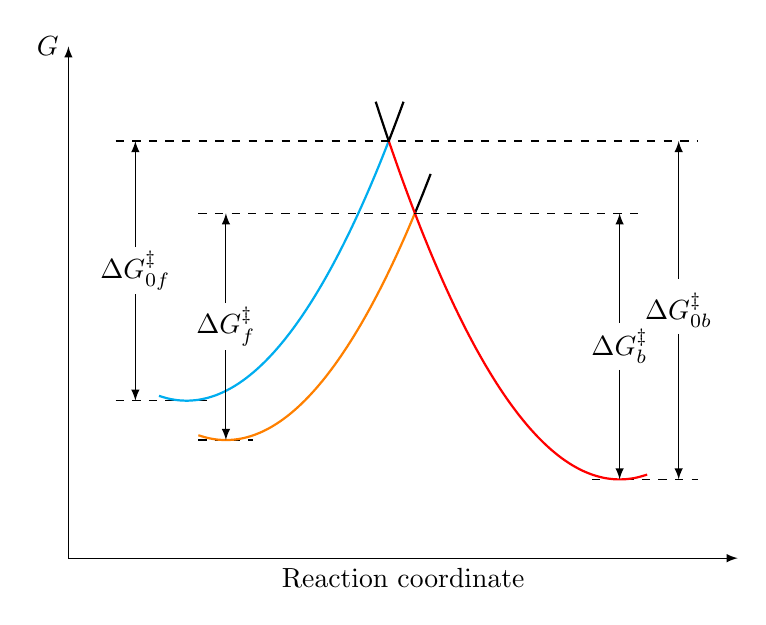
\begin{tikzpicture}
    \draw[-latex] (-1,0)--(7.5,0);
    \node[below] at (3.25,0) {Reaction coordinate};
    \draw[-latex] (-1,0)--(-1,6.5) node[left] {$G$};
    \draw[dashed] (-0.4,2)--(0.85,2);
    \draw[dashed] (0.65,1.5)--(1.35,1.5);
    \draw[dashed] (5.65,1)--(7,1);
    \draw[thick,cyan,domain=0.15:3.068] plot[smooth] (\x,{(\x-0.5)^2/2+2});
    \draw[thick,domain=3.068:3.2557] plot[smooth] (\x,{(\x-0.5)^2/2+2});
    \draw[thick,orange,domain=0.65:3.4] plot[smooth] (\x,{(\x-1)^2/2+1.5});
    \draw[thick,domain=3.4:3.6] plot[smooth] (\x,{(\x-1)^2/2+1.5});
    \draw[thick,red,domain=3.068:6.35] plot[smooth] (\x,{(\x-6)^2/2+1});
    \draw[thick,domain=2.9026:3.068] plot[smooth] (\x,{(\x-6)^2/2+1});
    \draw[dashed] (-0.4,5.29777)--(7,5.29777);
    \draw[dashed] (0.65,4.38)--(6.25,4.38);
    \node at (-0.15,3.6488) {$\Delta G^\ddagger_{0\text f}$};
    \draw[-latex] (-0.15,3.9488)--(-0.15,5.2977);
    \draw[-latex] (-0.15,3.3488)--(-0.15,2);
    \node at (1,2.94) {$\Delta G^\ddagger_{\text f}$};
    \draw[-latex] (1,3.24)--(1,4.38);
    \draw[-latex] (1,2.64)--(1,1.5);
    \node at (6.75,3.1488) {$\Delta G^\ddagger_{0\text b}$};
    \draw[-latex] (6.75,3.5488)--(6.75,5.2977);
    \draw[-latex] (6.75,2.8488)--(6.75,1);
    \node at (6,2.69) {$\Delta G^\ddagger_{\text b}$};
    \draw[-latex] (6,2.99)--(6,4.38);
    \draw[-latex] (6,2.39)--(6,1);
\end{tikzpicture}
\end{document}
    \end{center}
    其中蓝线为理论电势下\ce{Ox}与\ce{e^-}的Gibbs自由能,%
    橙线为实际电势下\ce{Ox}与\ce{e^-}的Gibbs自由能.%
    显然,在理论电势下,反应的历程为蓝线-红线,而在实际电势下,反应的历程为橙线-红线.\\
    我们现在将临近过渡态的区域放大,得到下图.
\end{derivation}
\end{document}